\clearpage
\section{Anchor loss analysis}
\subsection{1D waves}
\begin{flushleft}
  \textbf{Inputfile:}
  \ttt{\ttilde/hiqlab/models/tutorial/pml1d}\\
  \textbf{Lua features introduced:}
  \ttt{make\_material\_s, add\_block, set\_stretch, f0}\\
  \textbf{MATLAB features introduced:}
  \ttt{Mesh\_assemble\_R, harmonic\_state, plotfield1d, plotcycle1d},
  plotting the stretch function
\end{flushleft}
This example illustrates basic anchor loss
modeling using Perfect Matched Layers. Though
this problem is 1 dimensional, the idea extends
to the multidimensional case. 

Ideally we would like to simulate the situation
shown in part A of Figure \ref{fig:PropagatingWaves},
where a wave propagates into an infinite domain,
resulting in only outgoing waves. Computationally
we cannot model and infinite domain and must truncate
it at a finite length. Blindly applying a fixed boundary
condition at the end results in part B of Figure
\ref{fig:PropagatingWaves}, where we obtain unphysical
standing waves. By applying this method of PML on a 
layer close to the boundary as is shown in light gray in 
Figure \ref{fig:PropagatingWaves}, we are able to regain
the situation in A, where we again have propagating waves.
Waves propagating through the PML layer are exponentially
damped. If the PML layer and a parameter \ttt{f0} that
we mention later are chosen properly, the waves are fully
damped by the time they reach the boundary and produce 
close to zero wave reflections. 

To define this PML we assign the \ttt{stretch\_function} 
mentioned in section ?? to the elements that the PML 
region is defined. The form of the \ttt{stretch\_function}
that is applied for this 1D case is shown in 
Figure \ref{fig:1DPMLSchematic}. The actual equation is,
\begin{eqnarray}
\text{stretch\_function(x)}
&=& \text{max}\left(0, \text{f0} \frac{\text{x-xpml}}
                                      {\text{xrad-xpml}}\right)
\end{eqnarray}
which is a linear function that takes 0 at the initiation of
the PML and \ttt{f0} at the boundary. The performance of the 
PML depends on the length of the PML and parameter \ttt{f0} and
they can be selected heuristically as shown in paper ???. 
In general a long PML and large \ttt{f0} desired, though
increasing the length will increase computational costs and 
as will be seen in the example, increasing the \ttt{f0} without
increasing the mesh density of the elements degrades performance.
In MEMS applications a value of approximately 40 is observed to
give standard performance.
There exists a function in MATLAB named \ttt{estimate\_pml} which
does this. (See section on ????).

\begin{figure}[htbp]
  \begin{minipage}{0.45\linewidth}
  \centering
  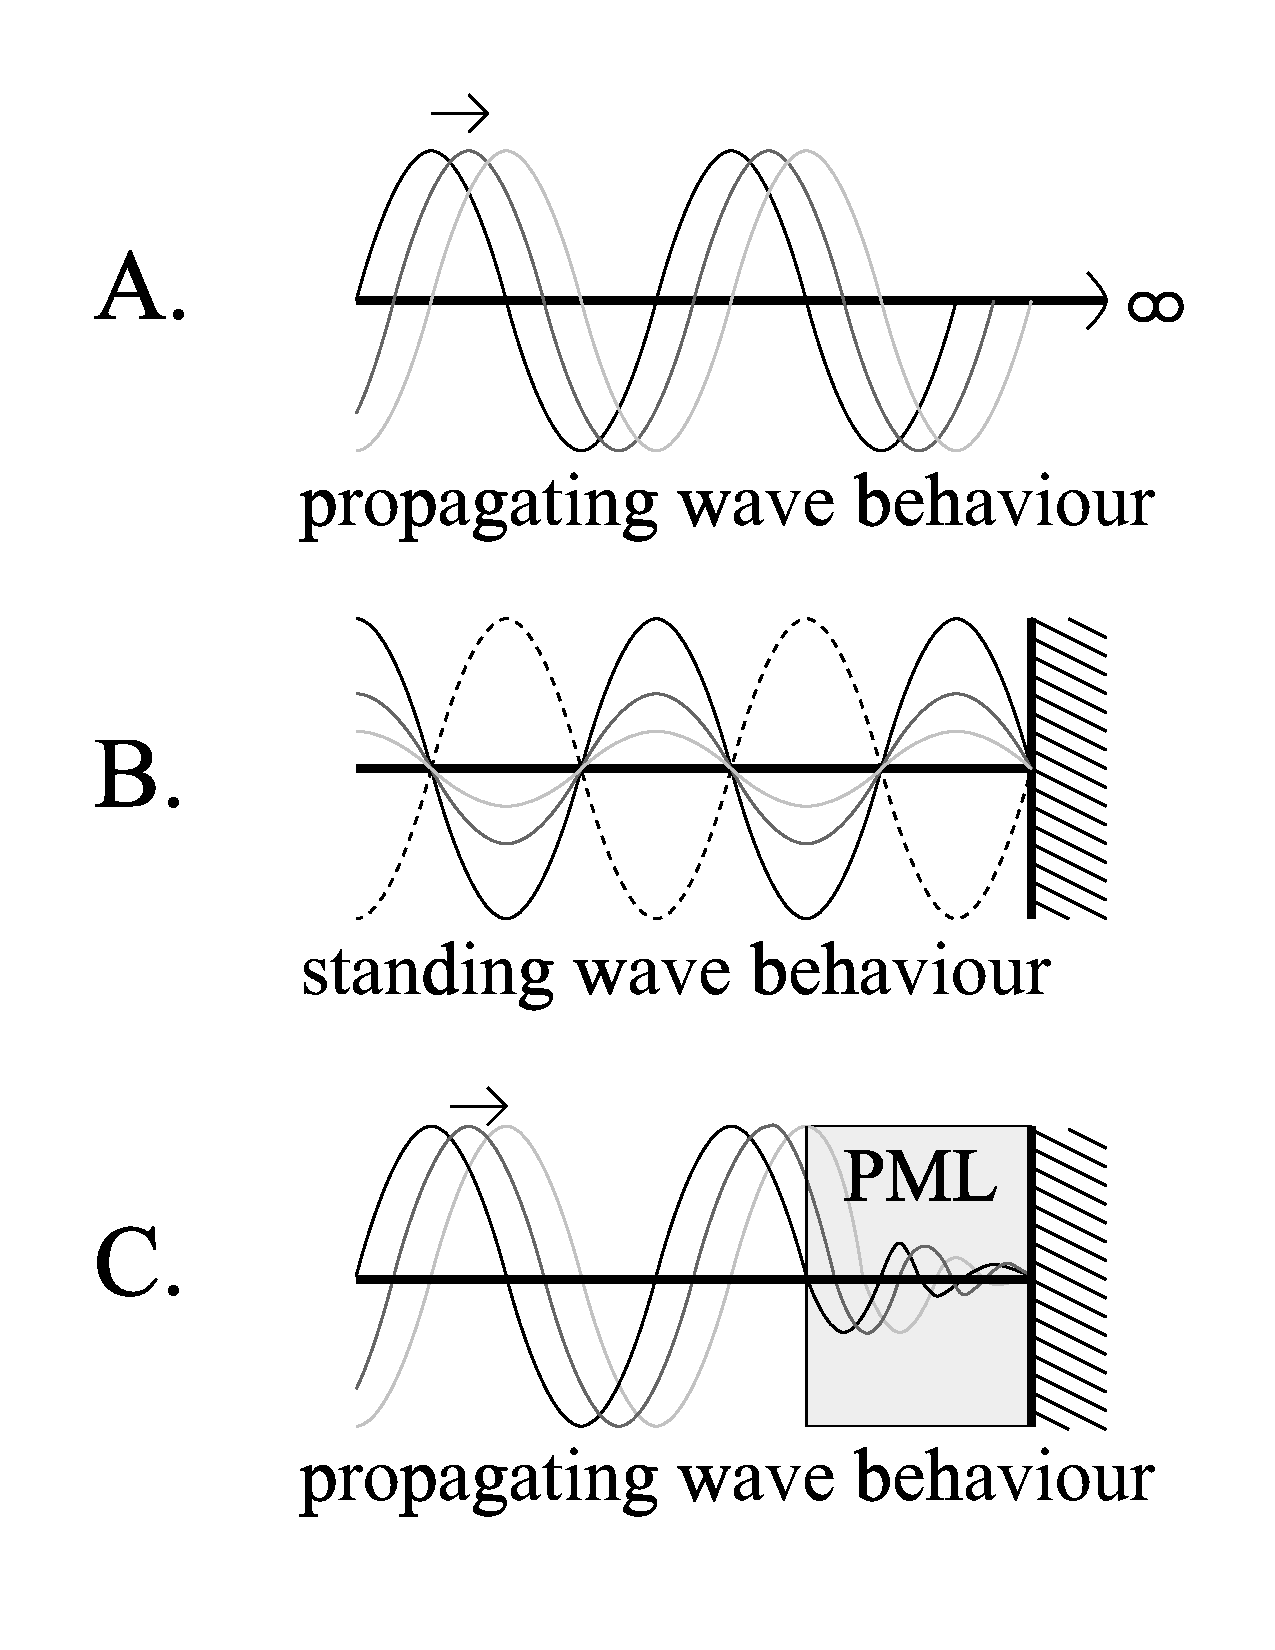
\includegraphics[trim = 0in 0in 0in 0in, clip, height=4in]{fig/propagatingwaves.pdf}
  \caption{Propagating Waves}
  \label{fig:PropagatingWaves}
  \end{minipage}
%\end{figure}
%\begin{figure}[htbp]
  \begin{minipage}{0.45\linewidth}
  \centering
  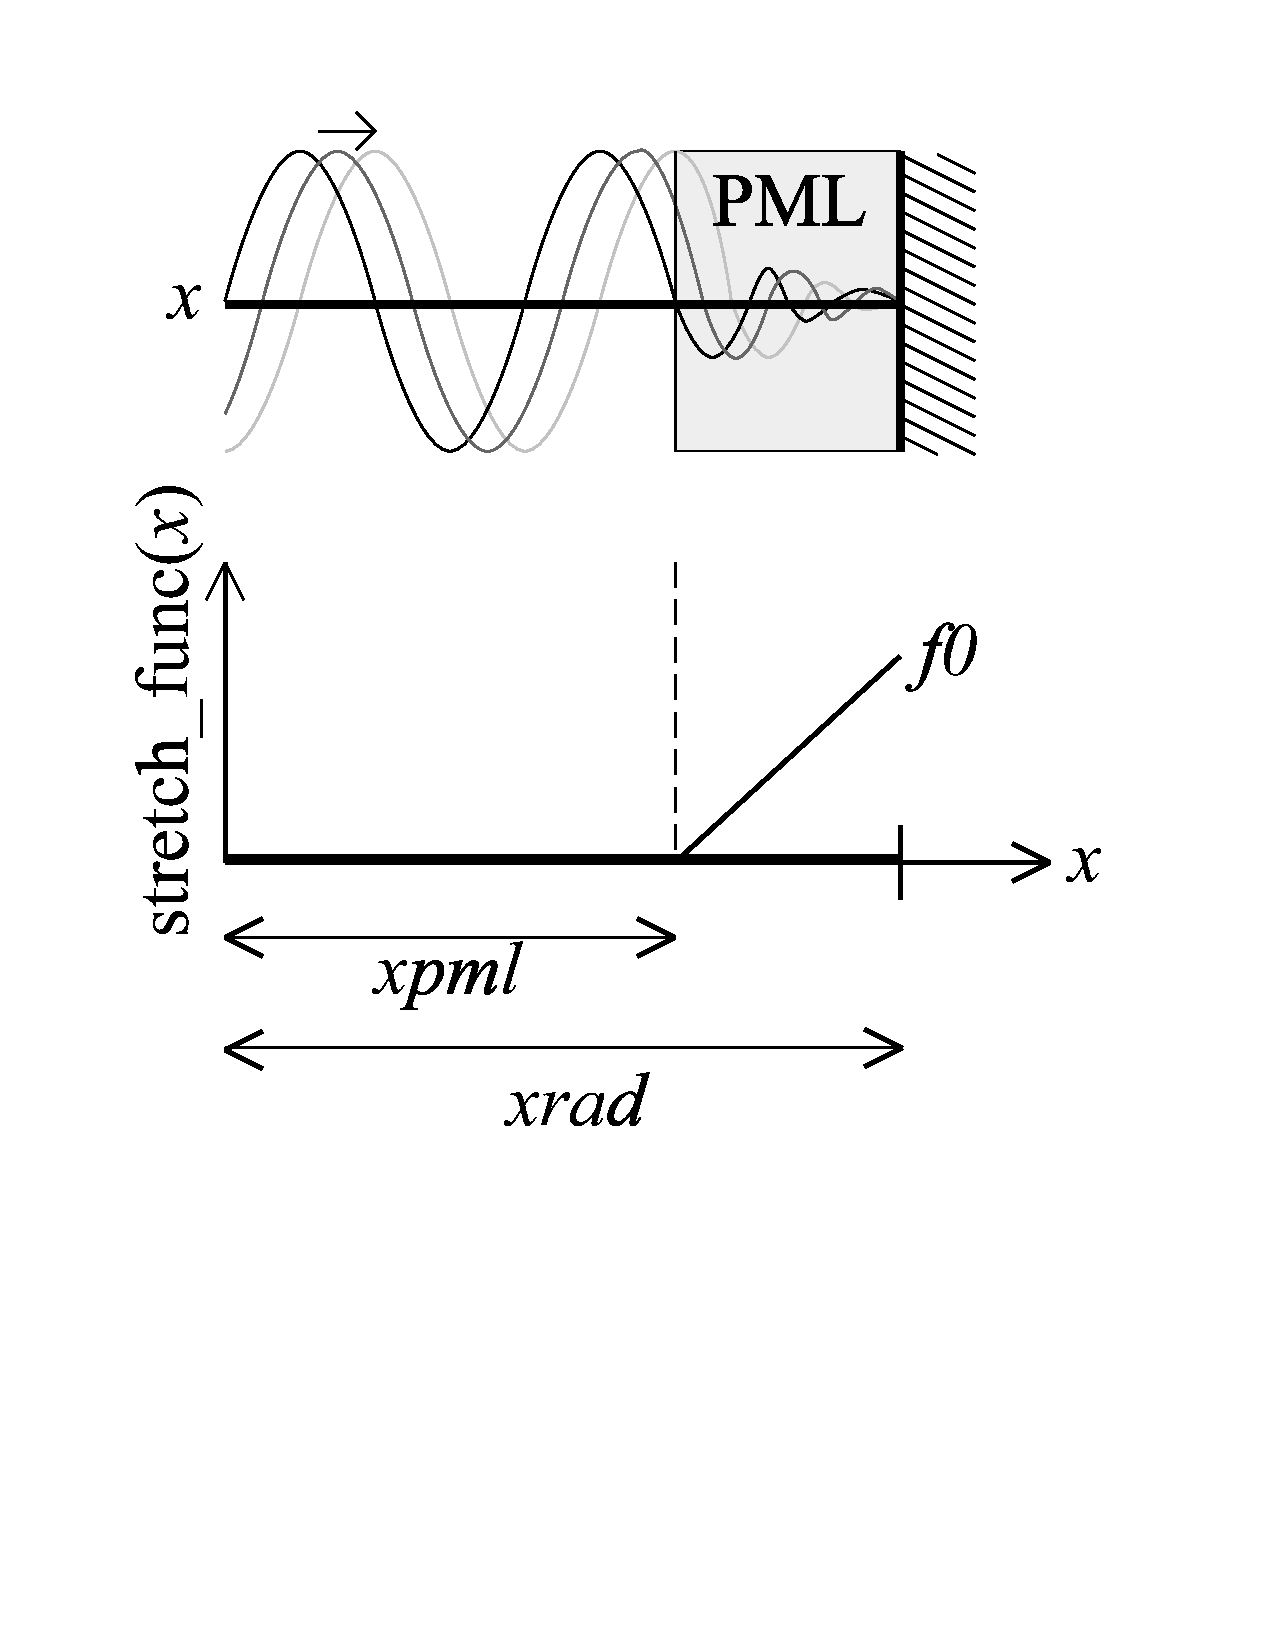
\includegraphics[trim = 0in 1in 0in 0in, clip, height=4in]{fig/1dpml.pdf}
  \caption{1D PML schematic}
  \label{fig:1DPMLSchematic}
  \end{minipage}
\end{figure}

\clearpage
\subsubsection*{Input file (LUA)}
\begin{flushleft}
  \textbf{Inputfile:}
  \ttt{\ttilde/hiqlab/models/tutorial/pml1d/pml1d.lua}\\
\end{flushleft}
\hspace{1in}
{\footnotesize
\listinginput[10]{1}{../../../models/tutorial/pml1d/pml1d.lua}
}

\clearpage
\begin{itemize}

  \item{\textbf{Construct element:}}
  First a material table \ttt{mtype} is defined. The
  required fields for a scalar static problem are 
  the Youngs modulus \ttt{E} and mass density \ttt{rho}.
  This material type, along with the string defining the 
  type of analysis is given to the command \ttt{make\_material\_s}
  which produces a scalar material.
  \begin{verbatim}
      etype = make_material_e( mtype, '1d');
  \end{verbatim}
  named \ttt{etype}.
  This element is used when elements are added to the \ttt{mesh}.

  \item{\textbf{Define PML parameter:}}
  The performance of the PML depends on the parameter \ttt{f0} and
  must be selected in accordance with the PML length.
  This value can be selected heuristically as shown in paper ???. 
  In general a long PML and large \ttt{f0} desired, though
  increasing the length will increase computational costs and 
  as will be seen in the example, increasing the \ttt{f0} without
  increasing the mesh density of the elements degrades performance.
  In MEMS applications a value of approximately 40 is observed to
  give standard performance.

  \item{\textbf{Define mesh using block command:}}
  The function \ttt{add\_block} adds a block of elements in the 
  range \ttt{[0, xrad]}. There are \ttt{num\_elem+1} nodes and 
  the elements have the order \ttt{order}.

  \item{\textbf{Define stretch function for PML:}}
  The stretch function to define the PML is defined here.
  The function must have the following structure, where
  the input is the physical coordinates of the mesh \ttt{x}, 
  and the output parameters are the stretching amount
  in each direction \ttt{sx}.
  \begin{verbatim}
     function stretch_function(x)
       -- compute sx
       return sx
     end
  \end{verbatim}

  \item{\textbf{Assign stretch function to element:}}
  The stretch function must be assigned to all elements that
  are defined as the PML region by the command,
  \begin{verbatim}
     etype:set_stretch(stretch_function)
  \end{verbatim}

  \item{\textbf{Define and assign boundary conditions:}}  
  A forced displacement boundary condition is set at the left end,
  and a fixed zero displacement boundary condition at the right end.

  Once the boundary condition function defined, it is assigned 
  to the mesh through the \ttt{set\_bc} command.

\end{itemize}

\clearpage
\subsubsection*{Solve harmonic problem (MATLAB)}
\begin{flushleft}
  \textbf{Inputfile:}
  \ttt{\ttilde/hiqlab/models/tutorial/pml1d/pml1d.m}\\
\end{flushleft}
\hspace{1in}
{\footnotesize
\listinginput[10]{1}{../../../models/tutorial/pml1d/pml1d.m}
}

\clearpage
Once the mesh is defined, the next step is to solve the problem.
This can be done both in Lua and MATLAB. Here we present the MATLAB
interface. 
The mesh obtained for this model is shown in 
Figure \ref{fig:PML1dMeshMATLAB}.

\begin{itemize}

  \item{\textbf{Define forcing frequency}}
  The computation conducted is a forced response. The 
  forcing frequency \ttt{w} is defined here in radians.

  \item{\textbf{Plot stretch function}}
  The stretch function should always be inspected for error.
  The function is visualized by the \ttt{plofield1d} command.
  This is done by assigning the string name of the stretch function, 
  in this case \ttt{stretch\_function}, to the field \ttt{cfields}
  in the optional structure \ttt{popt} and passing it to the 
  function \ttt{plotfield1d}. 

  \item{\textbf{Construct matrices and solve for harmonice displacements}}
  Here the matrices and forcing vectors are formed. The mathematical 
  structure of ordinary differential equation of the problem is
  \begin{eqnarray}
     \bfM\ddot{\bfu} + \bfK\bfu = \bff \nonumber
  \end{eqnarray} 
  By assuming harmonic displacements of the form,
  \begin{eqnarray}
     \bfu &=& \bfU \exp\left(iwt\right) \nonumber \\
     \bff &=& \bfF \exp\left(iwt\right) \nonumber
  \end{eqnarray}
  the equation,
  \begin{eqnarray}
    \bfU &=& \left(\bfK-w^2\bfM\right)^{-1}\bfF \nonumber
  \end{eqnarray}
  is obtained. 
  The function \ttt{harmonic\_state} solves this equation, given
  the forcing pattern $\bfF$.

  \item{\textbf{Display results}}
  The animation of the time-harmonic motion is displayed through
  the function \ttt{plotcycle1d}. (See section on plots for details).

\end{itemize}

\begin{figure}[htbp]
    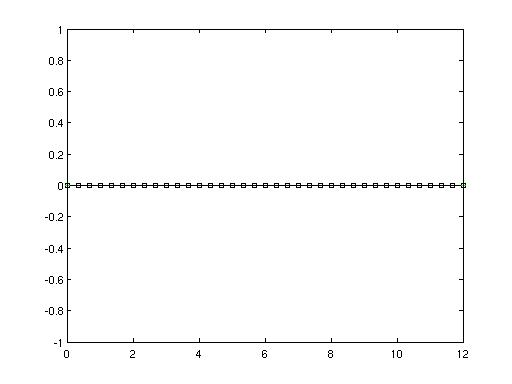
\includegraphics[width=\linewidth]{fig/pml1d_mesh_matlab.jpg}
    \caption{PML1d mesh from MATLAB}
    \label{fig:PML1dMeshMATLAB}
\end{figure}

\clearpage
\subsubsection*{Parametric study (MATLAB)}
Parametric study conducted by varying the variable 
\ttt{f0}. The stretch function values and mode shape plots
obtained for each case is shown in the figures.
For \ttt{f0=0} we see standing wave behavior, for \ttt{f0=40}
propagating wave behavior, and for \ttt{f0=4e6} again
standing wave behavior. 

\begin{figure}[htbp]
  \begin{minipage}{0.45\linewidth}
    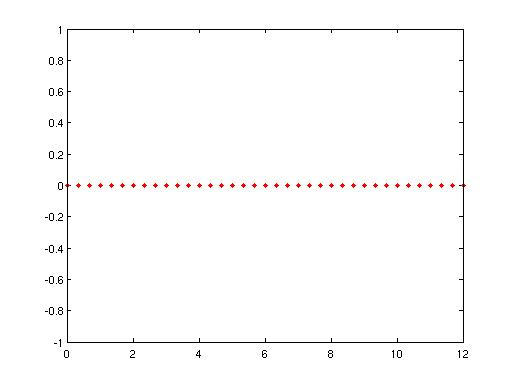
\includegraphics[width=\linewidth]{fig/pml1d_stretch0_matlab.jpg}
    \caption{PML1d stretch function from MATLAB(\ttt{f0=0})}
    \label{fig:PML1dStretchFunction0MATLAB}
  \end{minipage}
  \hfill
  \begin{minipage}{0.45\linewidth}
    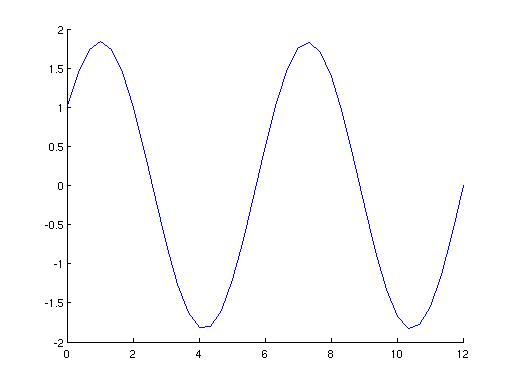
\includegraphics[width=\linewidth]{fig/pml1d_mode0_matlab.jpg}
    \caption{PML1d mode shape from MATLAB(\ttt{f0=0})}
    \label{fig:PML1dModeShape0MATLAB}
  \end{minipage}
  \begin{minipage}{0.45\linewidth}
    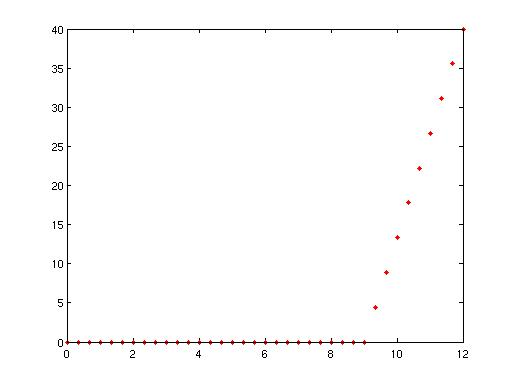
\includegraphics[width=\linewidth]{fig/pml1d_stretch40_matlab.jpg}
    \caption{PML1d stretch function from MATLAB(\ttt{f0=40})}
    \label{fig:PML1dStretchFunction40MATLAB}
  \end{minipage}
  \hfill
  \begin{minipage}{0.45\linewidth}
    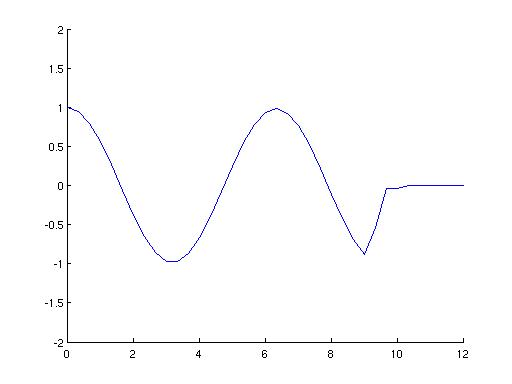
\includegraphics[width=\linewidth]{fig/pml1d_mode40_matlab.jpg}
    \caption{PML1d mode shape from MATLAB(\ttt{f0=40})}
    \label{fig:PML1dModeShape40MATLAB}
  \end{minipage}
  \begin{minipage}{0.45\linewidth}
    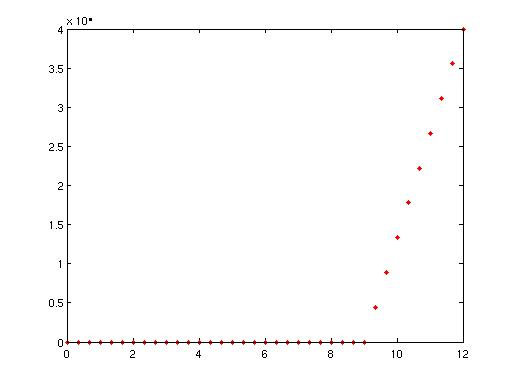
\includegraphics[width=\linewidth]{fig/pml1d_stretch4e6_matlab.jpg}
    \caption{PML1d stretch function from MATLAB(\ttt{f0=4e6})}
    \label{fig:PML1dStretchFunction4e6MATLAB}
  \end{minipage}
  \hfill
  \begin{minipage}{0.45\linewidth}
    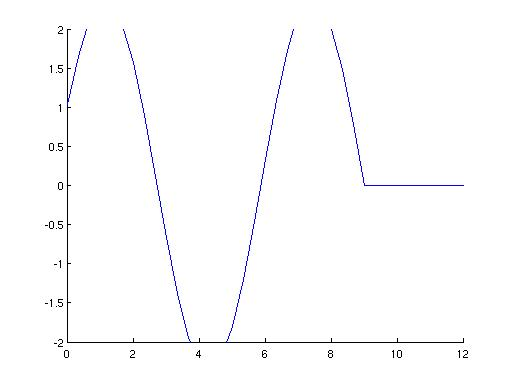
\includegraphics[width=\linewidth]{fig/pml1d_mode4e6_matlab.jpg}
    \caption{PML1d mode shape from MATLAB(\ttt{f0=4e6})}
    \label{fig:PML1dModeShape4e6MATLAB}
  \end{minipage}
\end{figure}

\clearpage
\subsection{2D waves}
\begin{flushleft}
  \textbf{Inputfile:}
  \ttt{\ttilde/hiqlab/models/tutorial/pml2d}\\
  \textbf{Lua features introduced:pml\_blocks2d}\\
  \textbf{MATLAB features introduced:}\\
  \ttt{plotfield2d, plotcycle2d}
\end{flushleft}
This example illustrates basic anchor loss
modeling using Perfect Matched Layers for the 
2D dimensional case. Two wave problems can
be considered for the 2 dimensional case, the
scalar wave and elastic wave. Both cases take
the same form for the stretch function required
to implement the PML. The functions are linear 
as in the 1 dimensional case, and their form
is shown in the schematic in Figure
\ref{fig:PML2dSchematic}. The mesh and stretch
function for both cases are shown in 
Figure \ref{fig:PML2dMeshMATLAB} and 
Figure \ref{fig:PML2dStretchFunctionMATLAB}.

\begin{figure}[htbp]
  \centering
  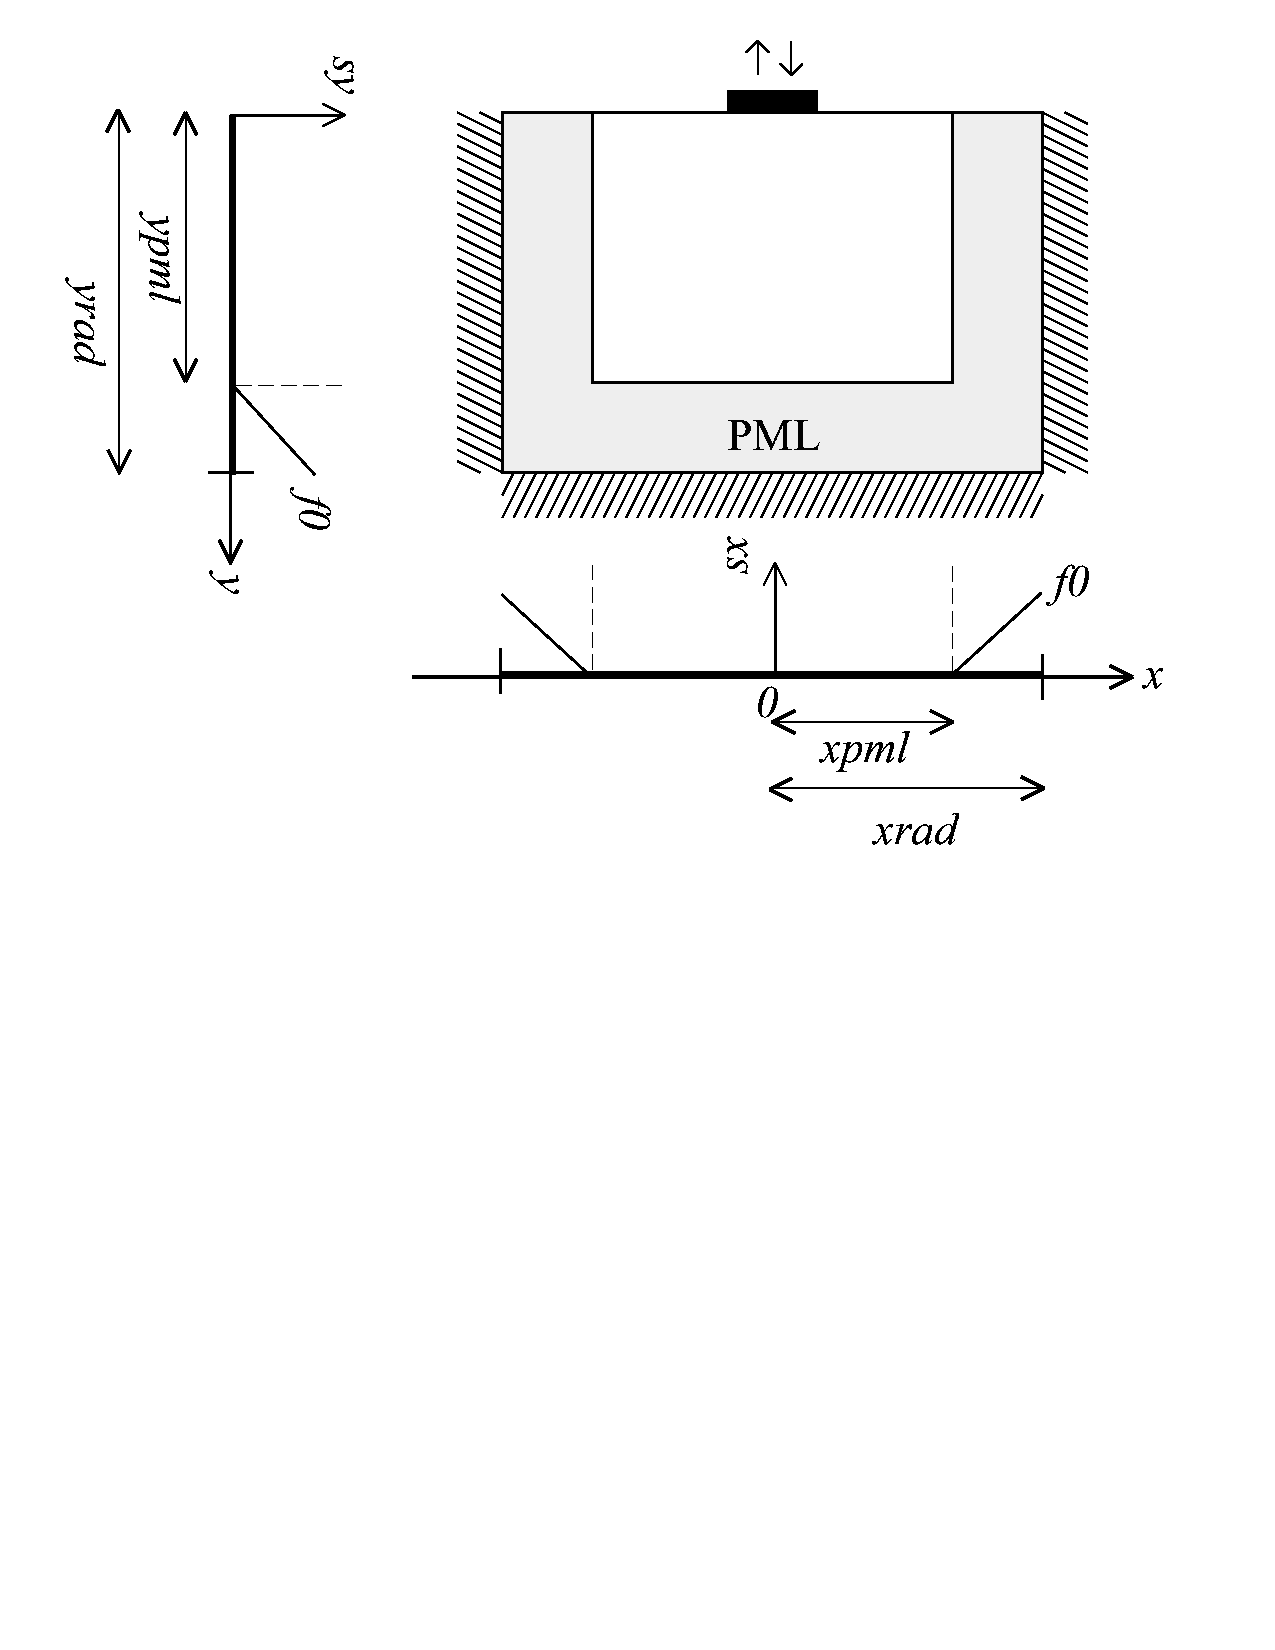
\includegraphics[trim = 0in 5in 0in 0in, clip, height=3.5in]{fig/2dpml.pdf}
  \caption{PML2d schematic}
  \label{fig:PML2dSchematic}
%\end{figure}
%\begin{figure}[htbp]
  \begin{minipage}{0.45\linewidth}
    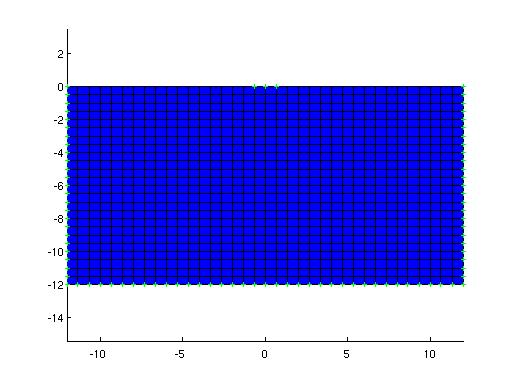
\includegraphics[width=\linewidth]{fig/pml2d_mesh_matlab.jpg}
    \caption{PML2d mesh from MATLAB}
    \label{fig:PML2dMeshMATLAB}
  \end{minipage}
  \hfill
  \begin{minipage}{0.45\linewidth}
    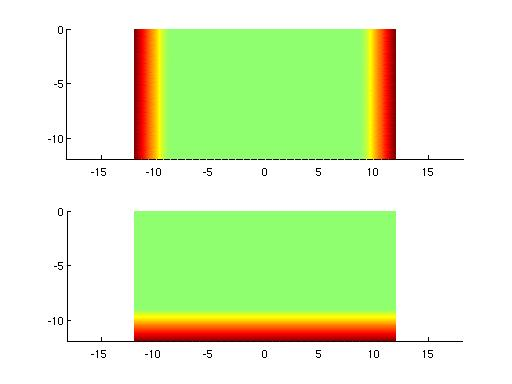
\includegraphics[width=\linewidth]{fig/pml2d_stretch_matlab.jpg}
    \caption{PML2d stretch function from MATLAB(\ttt{f0=40})}
    \label{fig:PML2dStretchFunctionMATLAB}
  \end{minipage}
\end{figure}

\clearpage
\subsubsection{Elastic waves in a half space}
\subsubsection*{Input file (LUA)}
\begin{flushleft}
  \textbf{Inputfile:}
  \ttt{\ttilde/hiqlab/models/tutorial/pml2d/pml2d.lua}\\
\end{flushleft}
\hspace{1in}
{\footnotesize
\listinginput[10]{1}{../../../models/tutorial/pml2d/pml2d.lua}
}

\clearpage
There is an additional file which uses the \ttt{pml\_blocks2d}
command to simply construct the pml anchor block.

\begin{itemize}

  \item{\textbf{Define Forcing parameters:}}
  Parameter \ttt{a} defines a pulling type of motion and 
  \ttt{b} a rocking type of motion. An example of 
  each is shown in the figures.

  \item{\textbf{Define stretch function for PML:}}
  The stretch function to define the PML is defined here.
  The function must have the following structure, where
  the input is the physical coordinates of the mesh \ttt{x,y}, 
  and the output parameters are the stretching amount
  in each direction \ttt{sx,sy}.
  \begin{verbatim}
     function stretch_function(x,y)
       -- compute sx,sy
       return sx,sy
     end
  \end{verbatim}
  The equations are,
  \begin{eqnarray}
  \text{sx}
        &=& \text{max}\left(0, \text{f0} \frac{\text{abs(x)-xpml}}{\text{xrad-xpml}}\right) \nonumber \\
  \text{sy}
        &=& \text{max}\left(0, \text{f0} \frac{\text{abs(y)-ypml}}{\text{yrad-ypml}}\right) \nonumber 
  \end{eqnarray}

  \item{\textbf{Assign stretch function to element:}}
  The stretch function must be assigned to all elements that
  are defined as the PML region by the command,
  \begin{verbatim}
     etype:set_stretch(stretch_function)
  \end{verbatim}

  \item{\textbf{Define and assign boundary conditions:}}  
  A forced displacement boundary condition is set at the middle with
  width 2, and fixed zero displacement boundary conditions are 
  defined on the bottom, left, and right edges.

  Once the boundary condition function is defined, it is assigned 
  to the mesh through the \ttt{set\_bc} command.

\end{itemize}

\clearpage
\subsubsection*{Input file using \ttt{pml\_blocks2d}(LUA)}
\begin{flushleft}
  \textbf{Inputfile:}
  \ttt{\ttilde/hiqlab/models/tutorial/pml2d/pml2d\_pmlblocks2d.lua}\\
\end{flushleft}
\hspace{1in}
{\footnotesize
\listinginput[10]{1}{../../../models/tutorial/pml2d/pml2d_pmlblocks2d.lua}
}

\clearpage
By using the function \ttt{pml\_blocks2d} this becomes,
\begin{itemize}

  \item{\textbf{Define pml block by function:}}
  The function creates a block of pml and returns the boundary 
  condition on the perimeter of the block \ttt{bc\_pmlfunc} and 
  the required stretch function \ttt{pml\_pmlfunc}. The input
  arguments are the nodes on the interface that the pml block is 
  to connect to. In this case nodes $(x,y) = (-1,0),(1,0)$. The
  first argument requires the x positions of these nodes and the 
  second the y positions. The third 2 denotes the degrees of freedom
  clamped at the edge by the boundary condition. In this case it is
  2 since it is a purely mechanical problem. The next two argument
  define the width and height of the pml block. \ttt{dpml} defines
  the depth of the pml layer from the fixed edges, \ttt{f0} is the
  damping parameter, \ttt{etype} the type of element used to construct
  the block, \ttt{order} is the order of interpolation, and 
  \ttt{densex,densey} are the approximate size of the elements in the 
  x and y direction.

  \item{\textbf{Set boundary condition}}
  In this case two boundary conditions must be set. One for the 
  forced boundary condition \ttt{bc\_function}, and the other for
  the anchor boundary condition \ttt{bc\_pmlfunc}. Thus a table
  bracketed by \{ and \} is passed to the function \ttt{set\_bc}.

\end{itemize}

\clearpage
\subsubsection*{Solve harmonic problem (MATLAB)}
\begin{flushleft}
  \textbf{Inputfile:}
  \ttt{\ttilde/hiqlab/models/tutorial/pml2d/pml2d.m}\\
\end{flushleft}
\hspace{1in}
{\footnotesize
\listinginput[10]{1}{../../../models/tutorial/pml2d/pml2d.m}
}

\clearpage
Once the mesh is defined, the next step is to solve the problem.
This can be done both in Lua and MATLAB. Here we present the MATLAB
interface. 
The mesh obtained for this model is shown in 
Figure \ref{fig:PML2dMeshMATLAB}.

\begin{itemize}

  \item{\textbf{Define forcing frequency}}
  The computation conducted is a forced response. The 
  forcing frequency \ttt{w} is defined here in radians.

  \item{\textbf{Define forcing pattern}}
  Additional parameters to define the forcing pattern are passed.
  The difference between these are shown in the figures.
  
  \item{\textbf{Plot stretch function}}
  The stretch function should always be inspected for error.
  The function is visualized by the \ttt{plofield1d} command.
  This is done by assigning the string name of the stretch function, 
  in this case \ttt{stretch\_function}, to the field \ttt{cfields}
  in the optional structure \ttt{popt} and passing it to the 
  function \ttt{plotfield2d}. 

  \item{\textbf{Display results}}
  The animation of the time-harmonic motion is displayed through
  the function \ttt{plotcycle2d}. (See section on plots for details).

\end{itemize}

\begin{figure}[htbp]
    \centering
    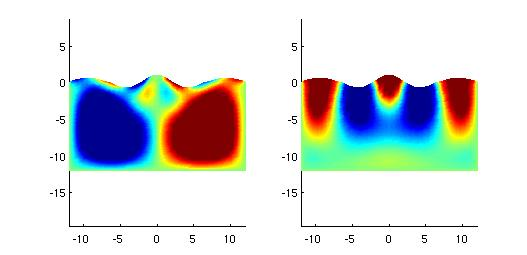
\includegraphics[width=0.7\linewidth]{fig/pml2d_mode0_matlab.jpg}
    \caption{PML2d mode shape from MATLAB(\ttt{f0=0})}
    \label{fig:PML2dModeShape0MATLAB}
    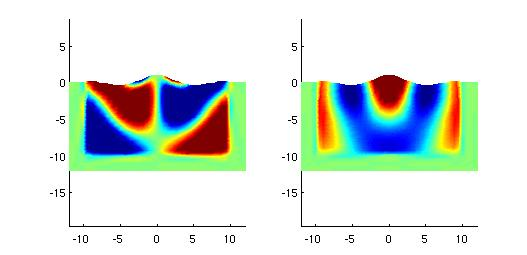
\includegraphics[width=0.7\linewidth]{fig/pml2d_mode40_matlab.jpg}
    \caption{PML2d mode shape from MATLAB(\ttt{f0=40})}
    \label{fig:PML2dModeShape40MATLAB}
    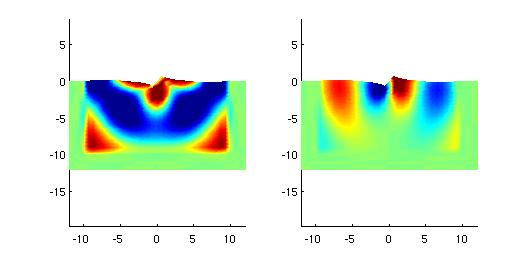
\includegraphics[width=0.7\linewidth]{fig/pml2d_mode40r_matlab.jpg}
    \caption{PML2d rocking mode shape from MATLAB(\ttt{f0=40})}
    \label{fig:PML2dModeShape40RockingMATLAB}
\end{figure}

\clearpage
\subsubsection{Scalar waves in a half space}
Since this is almost identical to the elastic case we
will only present the Lua input file and corresponding 
Matlab file.

\clearpage
\subsubsection*{Input file (LUA)}
\begin{flushleft}
  \textbf{Inputfile:}
  \ttt{\ttilde/hiqlab/models/tutorial/pml2d/pml2ds.lua}\\
\end{flushleft}
\hspace{1in}
{\footnotesize
\listinginput[10]{1}{../../../models/tutorial/pml2d/pml2ds.lua}
}

\clearpage
\subsubsection*{Solve harmonic problem (MATLAB)}
\begin{flushleft}
  \textbf{Inputfile:}
  \ttt{\ttilde/hiqlab/models/tutorial/pml2d/pml2ds.m}\\
\end{flushleft}
\hspace{1in}
{\footnotesize
\listinginput[10]{1}{../../../models/tutorial/pml2d/pml2ds.m}
}


\clearpage
\subsection{Axis-symmetric waves}
\begin{flushleft}
  \textbf{Inputfile:}
  \ttt{\ttilde/hiqlab/models/tutorial/pmlaxis}\\
  \textbf{Lua features introduced:}\\
  \textbf{MATLAB features introduced:}
\end{flushleft}
This example illustrates basic anchor loss
modeling using Perfect Matched Layers for the 
axis symmetric dimensional case. Two wave problems can
be considered for the 2 dimensional case, the
scalar wave and elastic wave. Both cases take
the same form for the stretch function required
to implement the PML. The functions are linear 
as in the 1 dimensional case, and their form
is shown in the schematic in Figure
\ref{fig:PMLAxisSchematic}. The mesh and stretch
function for both cases are shown in 
Figure \ref{fig:PMLAxisMeshMATLAB} and 
Figure \ref{fig:PMLAxisStretchFunctionMATLAB}.

\begin{figure}[htbp]
  \centering
  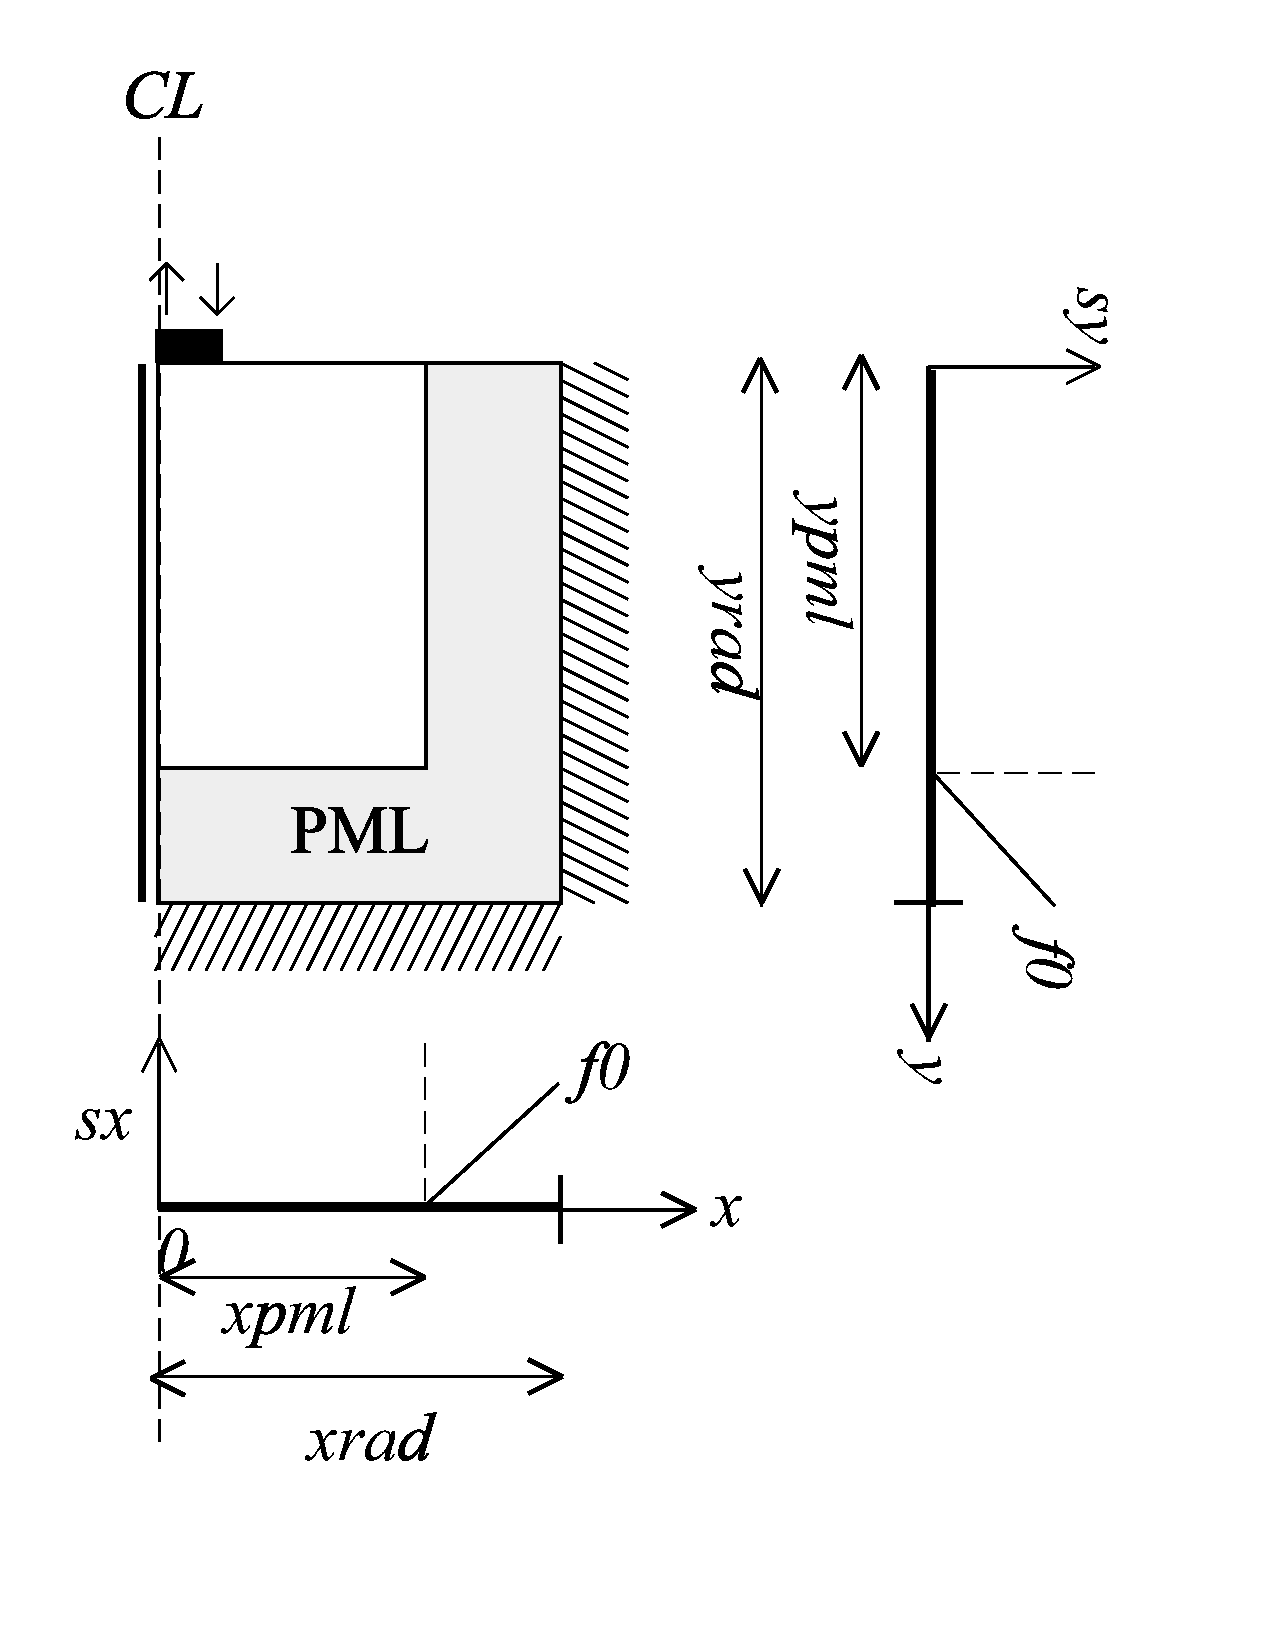
\includegraphics[trim = 0in 2in 0in 0in, clip, height=4in]{fig/2daxispml.pdf}
  \caption{PML Axis Schematic}
  \label{fig:PMLAxisSchematic}
%\end{figure}
%\begin{figure}[htbp]
  \begin{minipage}{0.45\linewidth}
    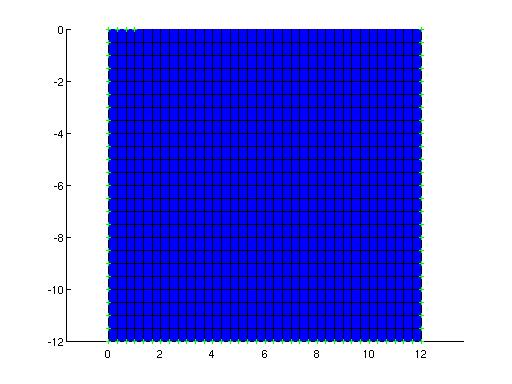
\includegraphics[width=\linewidth]{fig/pmlaxis_mesh_matlab.jpg}
    \caption{PMLAxis mesh from MATLAB}
    \label{fig:PMLAxisMeshMATLAB}
  \end{minipage}
  \hfill
  \begin{minipage}{0.45\linewidth}
    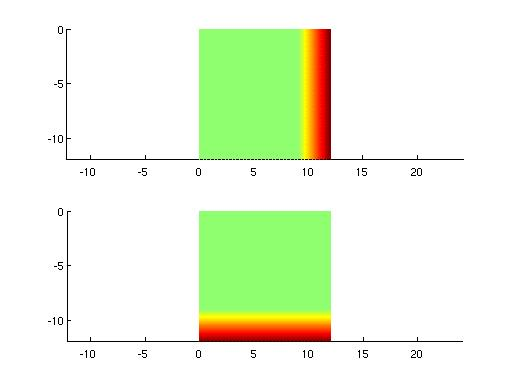
\includegraphics[width=\linewidth]{fig/pmlaxis_stretch_matlab.jpg}
    \caption{PMLAxis stretch function from MATLAB(\ttt{f0=40})}
    \label{fig:PMLAxisStretchFunctionMATLAB}
  \end{minipage}
\end{figure}


\clearpage
\subsubsection{Elastic waves in a half space}
Since this is almost identical to the 2d case we
will only present the Lua input file and corresponding 
Matlab file. 

\clearpage
\subsubsection*{Input file (LUA)}
\begin{flushleft}
  \textbf{Inputfile:}
  \ttt{\ttilde/hiqlab/models/tutorial/pmlaxis/pmlaxis.lua}\\
\end{flushleft}
\hspace{1in}
{\footnotesize
\listinginput[10]{1}{../../../models/tutorial/pmlaxis/pmlaxis.lua}
}

\clearpage
\subsubsection*{Solve harmonic problem (MATLAB)}
\begin{flushleft}
  \textbf{Inputfile:}
  \ttt{\ttilde/hiqlab/models/tutorial/pmlaxis/pmlaxis.m}\\
\end{flushleft}
\hspace{1in}
{\footnotesize
\listinginput[10]{1}{../../../models/tutorial/pmlaxis/pmlaxis.m}
}


\clearpage
\subsubsection{Scalar waves in a half space}
Since this is almost identical to the 2D case we
will only present the Lua input file and corresponding 
Matlab file. 

\clearpage
\subsubsection*{Input file (LUA)}
\begin{flushleft}
  \textbf{Inputfile:}
  \ttt{\ttilde/hiqlab/models/tutorial/pmlaxis/pmlaxis\_s.lua}\\
\end{flushleft}
\hspace{1in}
{\footnotesize
\listinginput[10]{1}{../../../models/tutorial/pmlaxis/pmlaxis_s.lua}
}

\clearpage
\subsubsection*{Solve harmonic problem (MATLAB)}
\begin{flushleft}
  \textbf{Inputfile:}
  \ttt{\ttilde/hiqlab/models/tutorial/pmlaxis/pmlaxis\_s.m}\\
\end{flushleft}
\hspace{1in}
{\footnotesize
\listinginput[10]{1}{../../../models/tutorial/pmlaxis/pmlaxis_s.m}
}

